\chapter{Opis projektnog zadatka}
		
		 U ovo moderno doba i vrijeme, kada su tehnološka sredstva uvijek nadomak ruke, nekolicina entuzijasta se dosjetila kako doskočiti u pomoć svom gradu. Naime, štete po cestama i javnim provršinama se ne smanjuju, ali to je upravo cilj jednog ovakvog projekta. \\
		
		 Ono što ovaj projekt nastoji ponuditi jest upravo jedno pravo suvremeno i efikasno rješenje pristupačno svima,a usmjereno samo prema jednoj stvari - otklanjanju štete javnih površina u gradu. Cilj projekta je svim ljudima omogućiti jednostavni pristup aplikaciji preko koje će moći prijavljivati uočena oštećenja javnih površina i cesta u područjima gradova čime sveukupno kumulira poboljšanje života u društvu.\\
		
		 Ukratko, tijek zamišljenih događaja je idući: Korisnik uoči oštećenu gradsku imovinu ili cestu te istu želi prijaviti gradskom uredu nadležnom za taj tip štete. Korisnik učitava našu aplikacuju te šalje prijavu sa određenim popunjenim podacima. Gradski ured dobiva obavijest o prijavi te kad istu riješi korisnik koji ju je prijavio dobiva obavijest da je ona razriješena. \\
		
		 Pri učitavanju početne stranice aplikacije korisniku je vidljiva karta, opcija za registraciju (ili prijavu), te opcija za podnošenje prijave. Regsistririani kao i neregistrirani korisnici imaju mogućnost slanja prijave, ali razlika je u tome što neregistrirani korisnik dobiva jedinstveni broj pomoću kojeg prati status prijave, registrirani korisnik uvijek može samo ući u povijest svojih prijava i vidjeti status svake podnesene
		
		 \underline{Neregistrirani korisnik} se u svakom trenutku može regitrirati, te pri registraciji trebe navesti iduće podatke:
		
		\begin{packed_item}
		\item Ime
		\item Prezime
		\item Korisničko ime
		\item E-mail
		\item Lozinku\\
		\end{packed_item}
		
		 \underline{Registrirani korisnici} se uvijek mogu prijaviti u sustav pomoću svog korisničkog imena i lozinke. Ako je korisnik prijavljen u sustav, ima mogućnost odjave ponuđenu u gornjem desnom kutu.
		\noindent Registrirani korisnici su podijeljeni na iduć uloge:
			\begin{packed_item}
			\item Klijent
			\item Administrator
			\item Gradski ured\\
			\end{packed_item}
			
			\underline{Klijent} na karti ima označene sve aktivne prijave. Pri pregledu prijava, prijave može filtrirati po tematici (tipu) i lokaciji. Pri predaji prijave, korisnik mora unijeti odgovarajuće podatke. Također korisniku nije zabranjeno mijenjanje vlastitih osobnih podataka ako vidi potrebu za tim.\\

 \underline{Prijava} koja se šalje u sustav se sastoji od atributa:
			\begin{packed_item}
			\item Naziv
			\item Kratki opis
			\item Geografske koordinate
			\end{packed_item}
			
			U slučaju da korisnik šalje prijavu koja je na obližnjoj lokaciji neke već druge prijave poslane u sustav sustav ga o tome obavještava  tako da mu izbacuje obližnju prijavu i ponudu mu opciju  nadovezivanja na tu istu u slučaju da korisnik uoči kako je to upravo ta prijava koju je on htio poslati.Uz sve to, korisnik ocionalno može poslati i sliku viđenog i potom sustav, u slučaju da nisu unesene koordinate, langitudu i longitudu izvlači sa meta podataka fotografije.\\
			
			  Web stranica koja  nudi sličnu uslugu, ali je bazirana na vandalizmu i isključivo grafitima u Londonu je: \\ \url{https://www.newham.gov.uk/publichealth-safety/graffiti-reporting-removal}, a izgled je na slici \ref{fig:promjene}.\\
			
			\begin{figure}[H]
			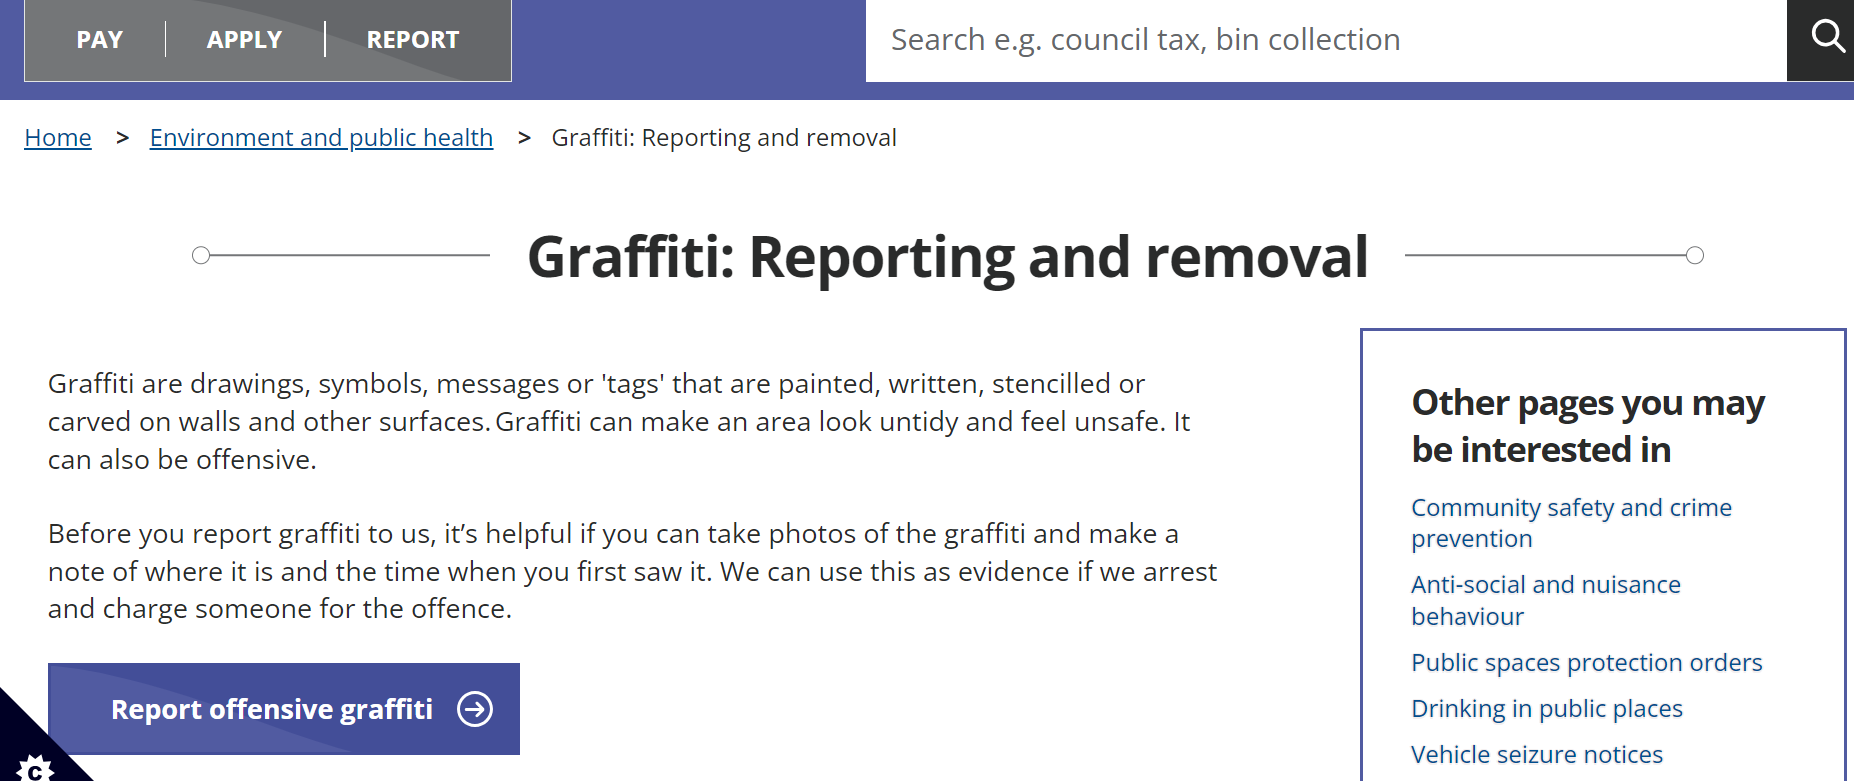
\includegraphics[scale=0.4]{slike/simular_page.PNG} %veličina slike u odnosu na originalnu datoteku i pozicija slike
			\centering
			\caption{Izgled navedene stranice}
			\label{fig:promjene}
		\end{figure}
		
		\underline{Administrator} je uloga koja ima najveće ovlasti. On je tu da kontrolira sve vezano za stranicu pa tako ima mogućnost uređivanja podataka pojedinih prijava kojen smatra nevaljalima kao i njihovo brisanje iz baze podatka. Pored toga, može brisati profile regsitriranih korsinika za koje procjeni da krše pravila ponašanja na aplikaciji, te potvrđuje ili opvrgava registraciju novih gradskih ureda za koje procijeni validnost.\\
		
		Uz navedene korisnike sustava, još postoje i \underline{gradski uredi/vijeća} koji primaju prijave na temelju tematike problema za koju su zaduženi. Tako će puknuće na cestama primati isključivo javni zavod za ceste, probleme sa zgradama će obrađivati ured za izgradnju i prostorno uređenje, probleme sa vodovodom ured za vodovod...  Dodatno, svaki gradski ured uvijek ima mogućnost  promjene statusa prijave koji će prijaviteljima omogućiti da jasno vide ukoliko je prijava razriješena ili nije. Uz to, ured može povezati one prijave koje korisnici nisu povezali ukoliko shvati da se radi o istom problemu iste tematike na konkretno bliskom podučju. Nadalje, ured prihavaća zahtjeve registriranih korisnika za ulazak u ured, to jest praticipaciju kako bi korisnik (koji je zaposlenik u tom uredu) dobio ovlasti gradskog ureda. Kreiranje (registracija) novih ureda u sustavu mora biti odobrena od strane administratora.\\
		
		Sustav će sve prijave obrađivati u stvarnom vremenu pa će korisnici u bilo kojem trenutku iamti uvid da li je npr. neko puknuće na cesti razriješeno te da li se tom cestom promet uopće može odvijati. Sličnu mogućnost nudi stranica HAK-a na idućoj adresi : \url{https://www.hak.hr/info/stanje-na-cestama/#prohodnost-cesta} na slici ref{hak}.\\
		
			
			\begin{figure}[H]
			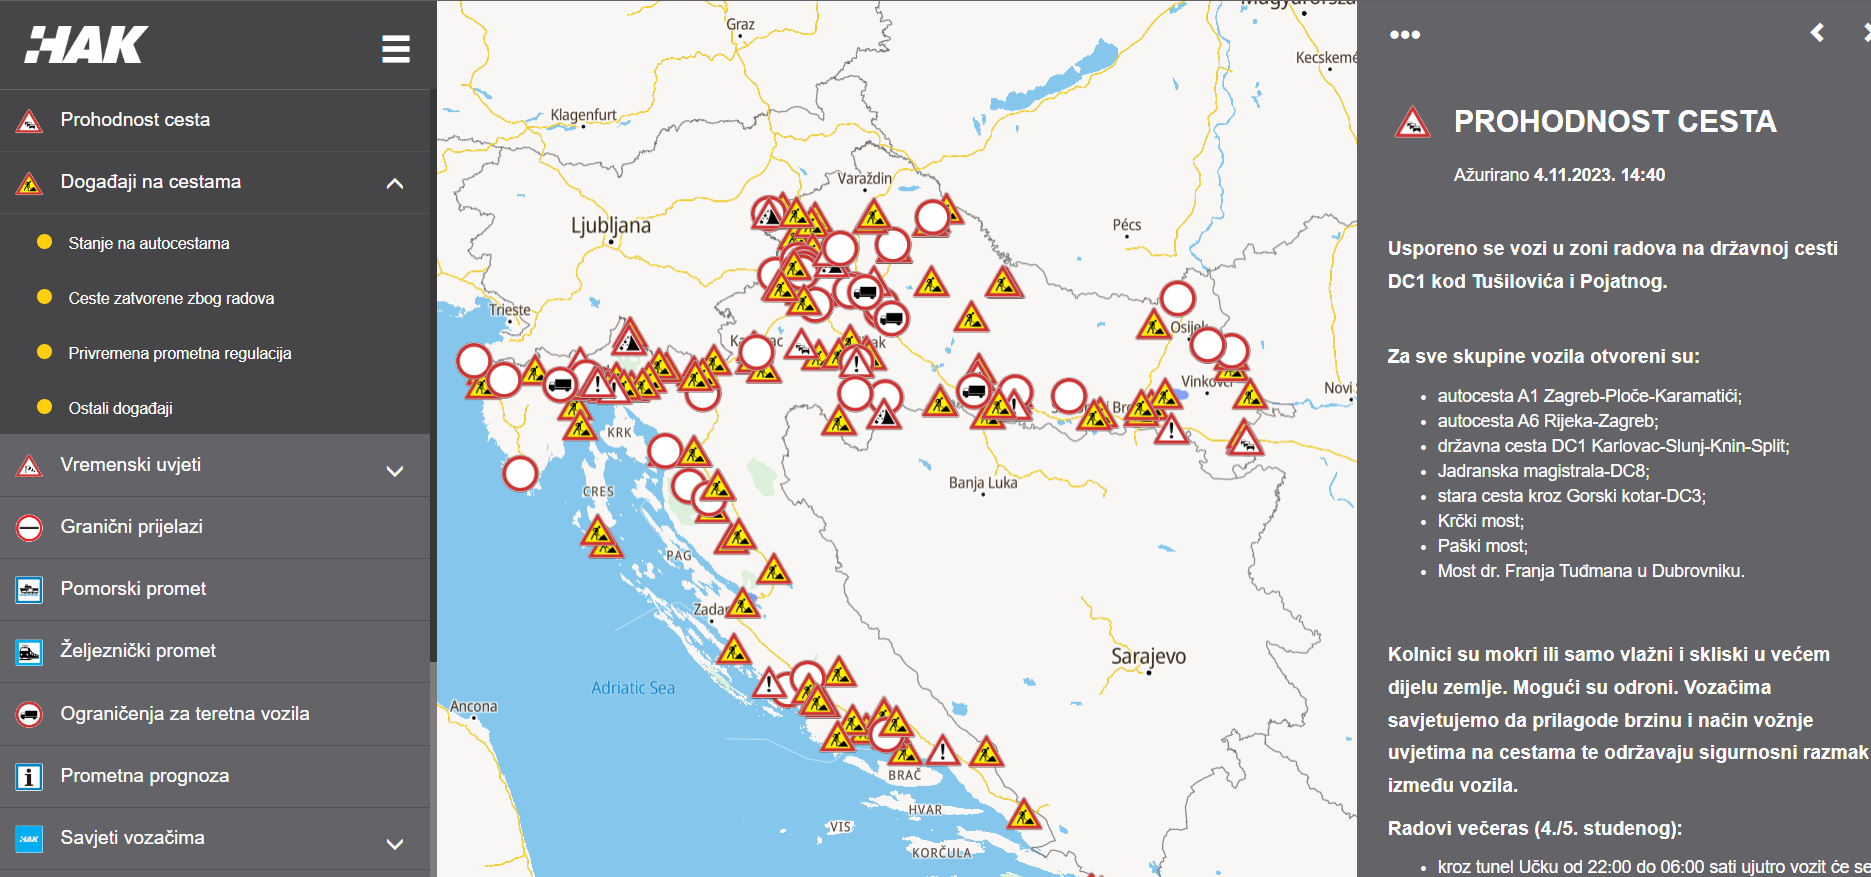
\includegraphics[scale=0.4]{slike/hak.PNG} %veličina slike u odnosu na originalnu datoteku i pozicija slike
			\centering
			\caption{HAK - stanje na cestama}
			\label{fig:hak}
		\end{figure}
		
		
		
		Ovakva aplikacije sama po sebi već ima klijentelu i predispozicije za uspješno korištenje i popularizaciju. Uz štete javnih površina i cesta moglo bi se dodati prijava za zastoj primjerice tramvaja na određenoj lokaciji (naravmo u gradovima gdje je tramvajski prijevoz omogućen) kako bi bilo vidljivo svim korisnicima aplikacije u stvarnom vremenu. Uz to moglo bi se područje aplikacije proširiti na prometne nesreće kako bi korisnici uz status da li je cesta zatvorena ili ne, mogli uz sliku procijeniti prohodnost iste. Neke vizualne stvari za korisnike koje se mogu još dodati bi bile gledanje tuđih profila, kao i dopisivanje porukama kako bi se doznale konkretnije informacije o prijavi od osobe koja je tu prijavu napravila. Besmisleno je izostaviti je Hrvatska turistička zemlja, te aplikaciji bi se još mogli dodati ostali osnovni jezici za inozemne korisnike. Kako bi se što više promoviralo prijavljivanje šteta, u aplikaciju bi se dala ugraditi neka online nagrađivanja; primjerice dostupnost povećanja levela i stjecanja points-a.